\section {Experimental setup}
 In the current SoLID design~\cite{solid_pcdr}, there are two configurations dedicated to the parity violation deep inelastic scattering (PVDIS) experiments and the semi-inclusive deep inelastic scattering experiments (SIDIS). We will use the same detector system as the approved SIDIS experiments, E12-10-006, E12-11-007, and E12-11-108, but with a minimum modification of the trigger design to include photon detection. In this section, we will briefly introduce the polarized $\mathrm{^{3}He}$ target and the SoLID detector system in the SIDIS configuration. A discussion of additional requirements for the new measurement will be also given and followed by a description of the conceptual trigger design. 
 
\subsection {Transversely Polarized $\mathrm{^{3}He}$ Target}
\begin{table}[!ht]
\centering
\begin{tabular}{|c|c|}
\hline
Target                       & $^3$He              \\\hline 
Length                       & 40 cm               \\\hline          
Target Polarization          & $\sim$60\%          \\\hline 
Target Spin Flip             & $\leq$20 mins       \\\hline 
Target Dilution              & 90\%  \\\hline
Effective Neutron            & 86.5\%  \\\hline
Target Polarimetry Accuracy  & $\sim$ 3\%          \\\hline
\end{tabular}
\caption{\footnotesize{Key Parameters of the $\mathrm{^{3}He}$ target.}}\label{table:target}
\end{table} 
The proposed measurement will utilize the same polarized $\mathrm{^{3}He}$ as E12-10-006~\cite{e12-10-006}. Such a target was successfully employed in E06-110, a 6~GeV SIDIS experiment in Hall A. The polarization direction is held by three sets of Helmholtz coils with a 25~Gauss magnetic filed. Both the transverse and longitudinal directions can be provided by rotating the magnetic field. The $\mathrm{^{3}He}$ gas with density of about 10~atm (at $0^{\circ}$) is stored in a 40~cm target cell made of thin glasses. With a 15~$\mu A$ electron beam, the neutron luminosity can be as high as $10^{36} cm^{-2}s^{-1}$. The in-beam polarization of 60\% was archived during the E06-110 experiment. Two kinds of polarimetry, NMR and EPR, were used to measure the polarization with relative 5\% precision. We have planed to improve the accuracy of the measurement to reach 3\%.

The target spin will be reversed for every 20 minutes by using the RF AFP technique. The additional polarization loss due to the spin reversal was kept at $<10~\%$ which has been taken into account in the overall 60\% in-beam polarization. A new method for spin reversal using filed rotation has been tested and was able to eliminate the polarization loss. Such an improvement will enable us to perform the spin-reversal in few minutes to reduce the target-spin-correlated systematics. The key parameters of the $\mathrm{^{3}He}$ target are summarized in Table~\ref{table:target}.
  
A collimator, similar to the one used in the E06-110, will be placed next to the target cell window to minimize the target cell contamination and to reduce the event rate. Several calibration targets will also be installed in this target system, including a multi-foil $^{12}C$ for optics study, a BeO target for beam tunning, and a reference target cell for dilution study and other calibration purposes.
  
\subsection {SoLID Spectrometer and Detectors} 
The solenoid magnet for SoLID will be based on the CLEO-II magnet built by Cornell University. The magnet is 3 meters long with the out diameter of 3 meters and the inner diameter of 1 meter. The field strength is greater than 1.35 Tesla with integrated BDL of 5 Tesla-meters. The fringe filed at the front end after shielding is less than 5 Gauss. In the SIDIS-configuration, the CLEO-II magnet provides 2$\pi$ acceptance in the azimuthal angle ($\phi$) and covers the polar angle ($\theta$) from 8$^{\circ}$ up to 24$^{\circ}$. The momentum acceptance is between 0.8 and 7.5~GeV/c and the resolution is about 2\%. 

\begin{figure}[!ht]
 \begin{center}
  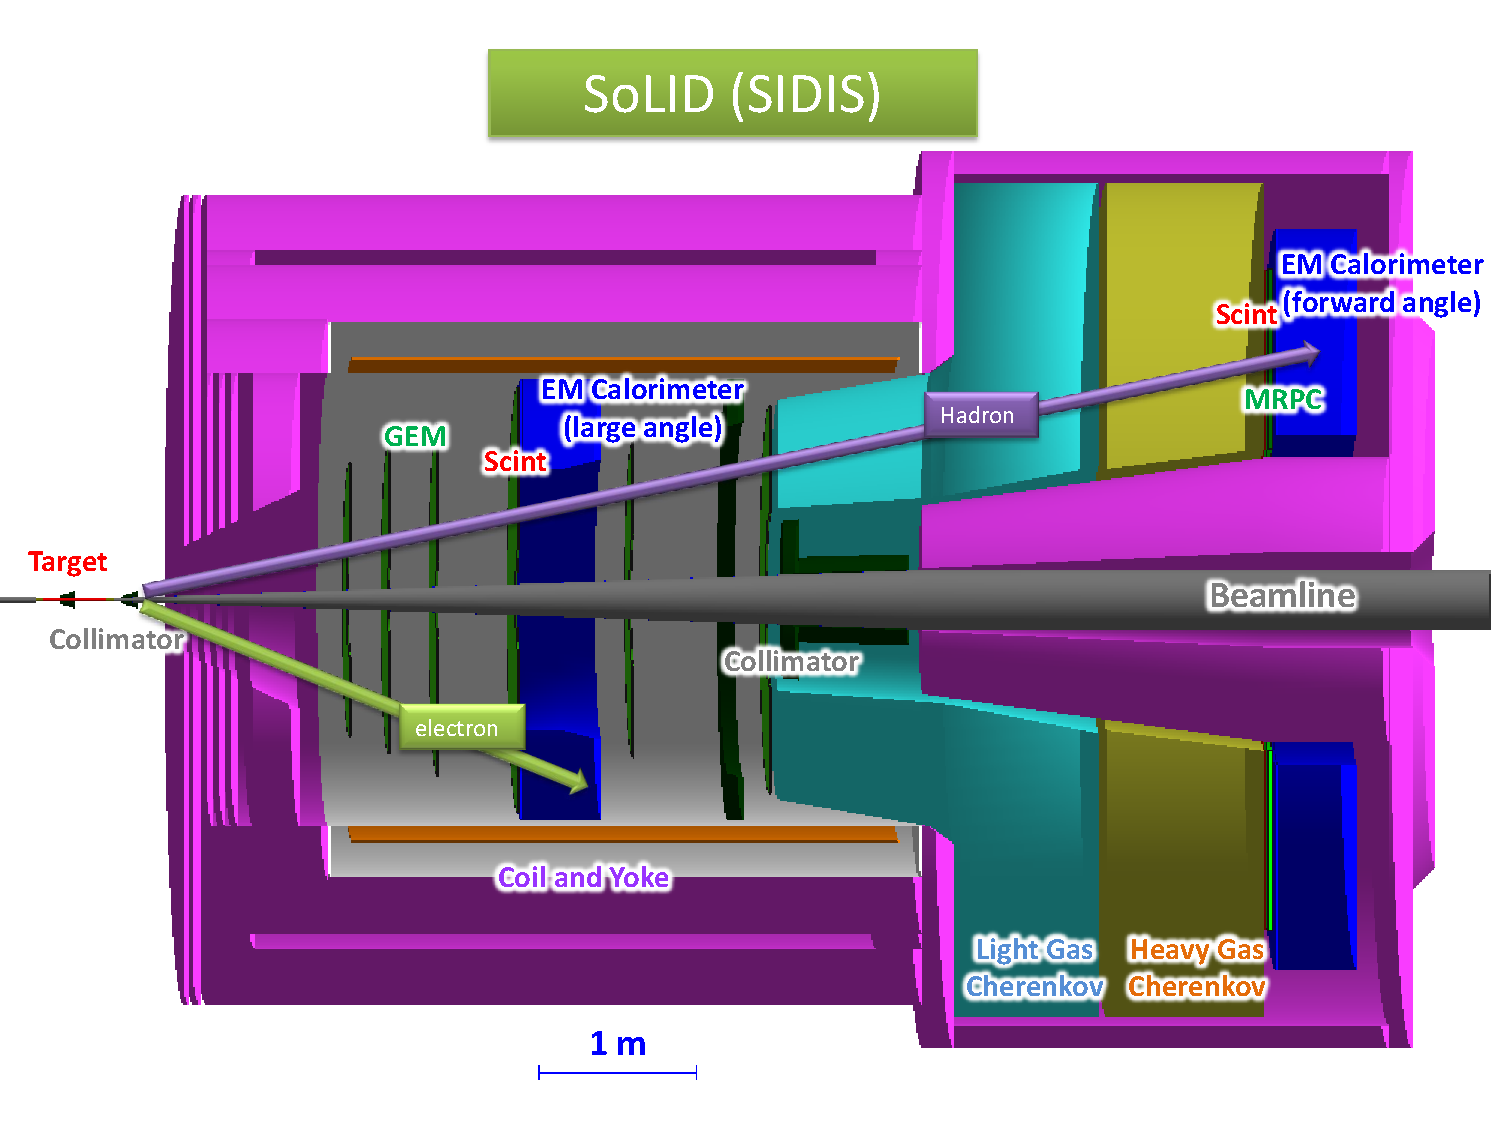
\includegraphics[width=0.8\textwidth]{./figures/SoLID_SIDIS_setup.pdf}
   \caption[The Detector Layout of the SoLID-SIDIS configuration]{\footnotesize{The Detector Layout of the SoLID-SIDIS configuration. The detector system includes six Gas Electron Multiplier (GEM) planes for charged particle tracking, two Scintillator Pad Detectors (SPD) followed by two Shashlyk sampling EM Calorimeters (EC) for energy measurement and particle identification, a Light Gas \v{C}erenkov Detector (LGC) for e-$\pi^{\pm}$ separation, a Heavy Gas \v{C}erenkov Detector (HGC) for $\pi^{\pm}$-$K^{\pm}$ separation, as well as a Multi-gap Resistive Plate Chamber (MRPC) for timing measurement. The first four GEM trackers, the first SPD (i.e. LASPD) and EC (i.e. LAEC) form the large-angle detection system for electron measurement. The forward-angle detection system, to measure electron and hadrons, is composed of all six GEM trackers, LGC, HGC, MRPC, the second SPD (i.e. FASPD) and the second EC (FAEC). The photon-detection in the large-angle is given by the veto-signal of the SPD in coincidence with the EC signal, where the photons in the forward-angle system will be triggered by the EC signal plus the veto-signals of LGC, SPD, and MRPC.}}
  \label{solid_sidis}
 \end{center}
\end{figure}
The layout of the SoLID detectors in the SIDIS-configuration is shown in Fig.~\ref{solid_sidis}. The detector system is divided into two parts for the forward-angle detection and the large-angle detection. Six Gas Electron Multiplier (GEM) tracking chambers will be used for charged particle tracking, where only four of them will be used for the large-angle detection. In each part, a Shashlyk-type sampling EM calorimeter (LAEC or FAEC) will measure the particle energy and identify electrons from hadrons, while a scintillator-pad detector (LASPD and FASPD) will be installed in front of each EC to reject photons. The forward-angle detectors will detect both the electrons and hadrons (mainly $\pi^{\pm}$). A light-gas \v{C}erenkov detector (LGC) and a heavy-gas \v{C}erenkov detector (HGC) will perform the $e/\pi^{\pm}$ and $\pi^{\pm}/K^{\pm}$ separation, respectively. The Multi-gas Resistive Plate Chamber (MRPC) will provide a precise timing measurement and serve as a backup of the FASPD on photon rejection. 

A more detailed discussion of the design, simulation, prototype-test of each detector is given in the SoLID preliminary conceptual design report (pCDR)~\cite{solid_pcdr}. 

\subsection{Additional Requirements for DVCS Measurement}
To use the existing SIDIS configuration for the DVCS measurement, it requires few minimum modifications. Both the scattered electrons and the photon will be detected to form the coincidence trigger. The photon-detection is not included in this configuration but can be easily added. In principle, the new measurement may be carried out along with the E12-10-006 by simply adding the photon trigger in addition to the electron and hadron triggers. New beam time will be requested in the actual proposal if more statistics are required to reach the proposed precision, or there are additional commissioning and calibration tasks needed, and last but not the least, the modification of the existing experimental configuration will bring significant impact to the SIDIS measurements. 
\begin{table}\centering
\begin{tabular}{|c|c|c|c|c|}
\hline
Experiments                             & SIDIS                 & DVCS  \\\hline
Reaction channel                        &  $(e,e'\pi^{\pm})$    & $(e,e'\gamma)$	\\\hline
Target                                  & $^3$He                & $^3$He 	\\\hline
Unpolarized luminosity                  & $\sim10^{37}$ cm$^{-2}$s$^{-1}$        & $\sim10^{37}$cm$^{-2}$s$^{-1}$	\\\hline 
Momentum coverage (GeV/c)               & 0.8-7.5               &0.8-7.5 	\\\hline
Momentum resolution                     &  $\sim$2\%            & $\sim$2\%	\\\hline
Polar angle coverage                    &  8$^{\circ}$-24$^{\circ}$                 &  8$^{\circ}$-24$^{\circ}$ 	\\\hline
Polar angle resolution                  & 0.6 mr                & 0.6 mr 	\\\hline
Azimuthal angle resolution              & 5 mr                  & 5 mr 	\\\hline
Target Vertex resolution                & 0.5~cm                & 0.5~cm \\\hline
 Energy resolution on ECs       & 5\%$\sim$10\%         & $\leq$5\%   \\\hline
 Position resolution on ECs     & 1~cm on x and y       & $\leq$1~cm on x and y   \\\hline
Trigger type                            & Coincidence $e^-+\pi^{\pm}$ & Coincidence $e^-+\gamma$\\\hline
Expected DAQ rates                      &  $<$100 kHz           &  $<$100 kHz 	\\\hline
Backgrounds                             & (e,$\pi^-\pi^{\pm}$)  &$(e,e'\pi^{0})$ \\
                                        &   (e,e'K$^\pm$)       &	\\\hline
Major requirements                      &  Radiation hardness   & Radiation hardness	\\
                                        &  DAQ                  & DAQ      \\
                                        &  Kaon Rejection       & Pion Rejection	\\
                                        &                       & Energy resolution  \\\hline
\end{tabular}
\caption{\footnotesize{Summary of Key Parameters for DVCS Measurement compared with SIDIS Experiments.}}\label{table:program_summary}
\label{table:key_par_sidis_dvcs}
\end{table} 

Since the recoil neutrons will not be detected, we will need to reconstruct the neutron missing mass spectrum to make sure the exclusivity of the measurement. On top of the similar hardware requirements as the SIDIS experiments, the DVCS measurement has greater demand on the detector resolutions. For electrons, the GEM tracking reconstruction is able to achieve very good accuracy on determining the momentum ($\sim$2\%) and the angles ($\sim 0.6~mrad$ on $\theta_{e}$ and $\sim 5.0~mrad$ on $\phi_{e}$). On the other hand, the precision of the photon measurement, however, have to rely on the performance of the ECs. The photon's angular resolutions are determined by the position resolutions of the EC cluster reconstruction, as well as the vertex resolution on the target which is given by the tracking reconstruction of electrons. The current design goal is to reach $\sim 1.0~cm$ precision on both the x- and y- directions on the EC plane. The cluster reconstruction will also determine the photon energy resolution within the range of $5\%\sim 10~\%$. Based on the experience from the Hall A DVCS experiments, a minimum requirement of the energy resolution for photon-detection should be less than $5\%/\sqrt{E}$. To perform the DVCS measurement, it is desired to improve the photon's energy resolution by optimizing both the EC design and the cluster reconstruction. 

Furthermore, the DVCS measurement will suffer from a large contamination by the $e+n\rightarrow e+n'+\pi^{0}$ reaction since a $\pi^{0}$ decays into two photons and the $n'+\gamma$ system mixes in the neutron spectrum. We plan to detect the two-photon events within the acceptance and remove the reconstructed $\pi^{0}$ background. The current EC and DAQ designs should be able to identify two-photon events but further investigation of the performance is required.  

Table~\ref{table:key_par_sidis_dvcs} summarizes the key parameters of the detector system in the SIDIS configuration for both the SIDIS and DVCS measurements. 

\subsection{Trigger Design}
\begin{figure}[!ht]
 \begin{center}
  \includegraphics[width=0.8\textwidth]{./figures/dvcs_trigger.pdf}
   \caption[A sketch map of the DVCS trigger design]{\footnotesize{A sketch map of the DVCS trigger design. At the large-angle part (LA), the electron trigger is formed by the ``AND`` of the LAEC signal and the LASPD signal, while the photon trigger is the coincidence signal of the LAEC signal and the veto-signal from the LASPD. Similarly, at the forward-angle part (FA), the electron trigger is the ''AND`` of the LGC, FASPD, MRPC and FAEC, and the photon trigger comes from the FAEC signal in coincident with the veto-signals of all other three detectors. Two coincidence signals are formed in the end to provide the event triggers from LA and FA.}}
 \label{dvcs_trigger}
\end{center}
\end{figure}
The DVCS events will be recorded with the coincidence trigger of the scattered electron and the photon. Both the large-angle detectors and forward-angle detectors can detect these particles at the same time, so two coincidence triggers will be created and sent to the DAQ system.  In principle, the DVCS triggers will be similar to the SIDIS trigger, but only the hadron triggers will be replaced by the photon triggers. If the new experiment runs together with E12-10-006, we will simply add two more triggers types on top of the existing SIDIS triggers. Fig.~\ref{dvcs_trigger} shows a sketch map, in a simplified way, to compose the electron and photon single-triggers, and the coincidence triggers. The actual trigger design will be far more complicated, and the detailed discussion of the trigger and DAQ design has been given in the SoLID pCDR~\cite{solid_pcdr}.
